\documentclass{article}
\usepackage{graphicx}
\usepackage{amsmath}
\usepackage{float}
\usepackage{hyperref}

\title{Esperienza di ottica}
\author{Alessandro Di Meglio \\ Francesco Angelo Fabiano Antonacci}
\date{\today}
\begin{document}

\maketitle
\section{Scopo dell'esperienza}
L'esperienza è suddivisa in due parti:

\begin{enumerate}
\item Misura dell'indice di rifrazione del plexiglas;
\item misura della focale di una lente divergente.

\end{enumerate}

\section{Cenni teorici}

Dalla legge di Snell, assumendo che l'indice di rifrazione dell'aria sia approssimabile a 1, otteniamo la seguente relazione:

	\begin{equation}
		n=\frac{sin\theta_i}{sin\theta_r}
			\label{eq:snell}
	\end{equation}

Dove n è l'indice di rifrazione del plexiglas, $\theta_i$ è l'angolo incidente del raggio e  $\theta_r$ è l'angolo  rifratto del raggio.


Sarà usata la seguente legge per fare i fit:
		\begin{equation}
				\sin{\theta_i}=n\sin{\theta_r}+q
							\label{eq:lin}
		\end{equation}
Dove si desidera che q sia compatibile con 0.


Data una lente la relazione tra $f$, ossia la distanza focale della lente, $p$ ,la distanza tra il centro della lente e la sorgente luminosa, e $q$ , la distanza tra il centro della lente e l'immagine messa a fuoco, è la legge dei punti coniugati:

\begin{equation}
\frac{1}{f}=\frac{1}{p}+\frac{1}{q}
\label{eq:pcon}
\end{equation}

Ponendo $\frac{1}{p}=x$ ,  $\frac{1}{q}=y$ e $\frac{1}{f}=c$ otteniamo la seguente relazione:
\begin{equation}
y=c-mx
\label{eq::)}
\end{equation}
Dove $m=1$.


 

\section{Apparato strumentale}


\subsection{Materiale Utilizzato}


\begin{itemize}

\item Banco ottico con sorgente luminosa;
\item semicilindro di plexiglas;
\item carta quadrettata;
\item cassetta di lenti;
\item supporto per il plexiglas.

\end{itemize} 

\subsection{Misure di lunghezza}

Le misure prese con il metro a nastro avranno come incertezza la deviazione standard della distribuzione uniforme sull'ampiezza della risoluzione ($1$[mm]).

Le misure relative al plexiglas sono state prese sulla carta quadrettata in unità arbitrarie, avranno come incertezza la deviazione standard della distribuzione uniforme sull'ampiezza della risoluzione ($1$[u.a.]) .

\section{Descrizione delle misure}

\subsection{Misura indice di rifrazione plexiglas}
 
E' stato orientato il semicilindro di plexiglas sulla carta quadrettata in modo tale che il raggio luminoso della sorgente passasse dal centro della faccia piana del semicilindro in modo tale che il raggio di luce venisse rifratto solo una volta. 
Sono state prese più misure delle lunghezze dei cateti proporzionali ai seni  degli angoli che il raggio di luce tracciava sulla carta a diverse orientazioni.


\subsection{Misura focale di una lente divergente}

Grazie a una lente convergente, è stato messo a fuoco su uno schermo un raggio di luce. 
E' stata posta più volte una lente divergente tra lo schermo e la lente convergente a distanze arbitrarie. 
Ogni volta è stato messo a fuoco sullo schermo il raggio di luce ed è stata misurata la distanza tra lente divergente e schermo. 

\subsection{Incertezze delle misure dirette}


\subsubsection{Incertezza sulle misure per stimare l'indice del plexiglas}

Per misurare i cateti dei seni degli angoli sono stati contati i quadretti sulla carta quadrettata.
Come incertezza è stata adottata la  deviazione standard della distribuzione lineare ampia come la risoluzione dello strumento.

\subsubsection{Incertezza sulle misure delle posizioni delle lenti nella misura della focale della lente}

Come incertezza sulla distanza $p$ tra schermo e lente divergente è stata considerata la deviazione standard della distribuzione uniforme su un intervallo largo quanto lo spessore della lente divergente: $\sigma_p=0.001$[m].
 Come incertezza sulla distanza $q$ tra schermo è stato necessario stimare l'ampiezza degli intervalli di messa a fuoco e sull'ampiezza massima fare la deviazione standard della distribuzione uniforme.

\section{Analisi dei dati}
 
\subsection{Misura indice rifrazione plexiglas}

Non essendo trascurabile l'errore sulla variabile indipendente sono stati usati gli errori efficaci.
E' stato fatto un algoritmo di best-fit con i minimi quadrati per la legge($\ref{eq:lin}$).
Desideriamo che l'intercetta sia compatibile con lo $0$: così che l'equazione(\ref{eq:snell}) sia soddisfatta.
Sono riportati in tabella($\ref{tab:plex}$) i risultati dell'algoritmo di best-fit.
In figura($\ref{fig:plex}$) sono riportati i dati raccolti e la previsione del modello teorico con i parametri ottenuti dall'algoritmo di best-fit.
In figura ($\ref{fig:plexres}$) è riportato il grafico dei residui.


\begin{table}[H]
		\centering
			\begin{tabular}{|cc|}
				\hline
				$n_{plexiglass}$ & $1.51 \pm 0.03$\\
				$q[u.a.]$ & $0.2 \pm 0.2$\\
				\hline
			\end{tabular}
		\caption{Valori ottenuti dall'algoritmo di best-fit per la legge (\ref{eq::)}).}
		\label{tab:plex}
		
\end{table}


\begin{figure}[H]
	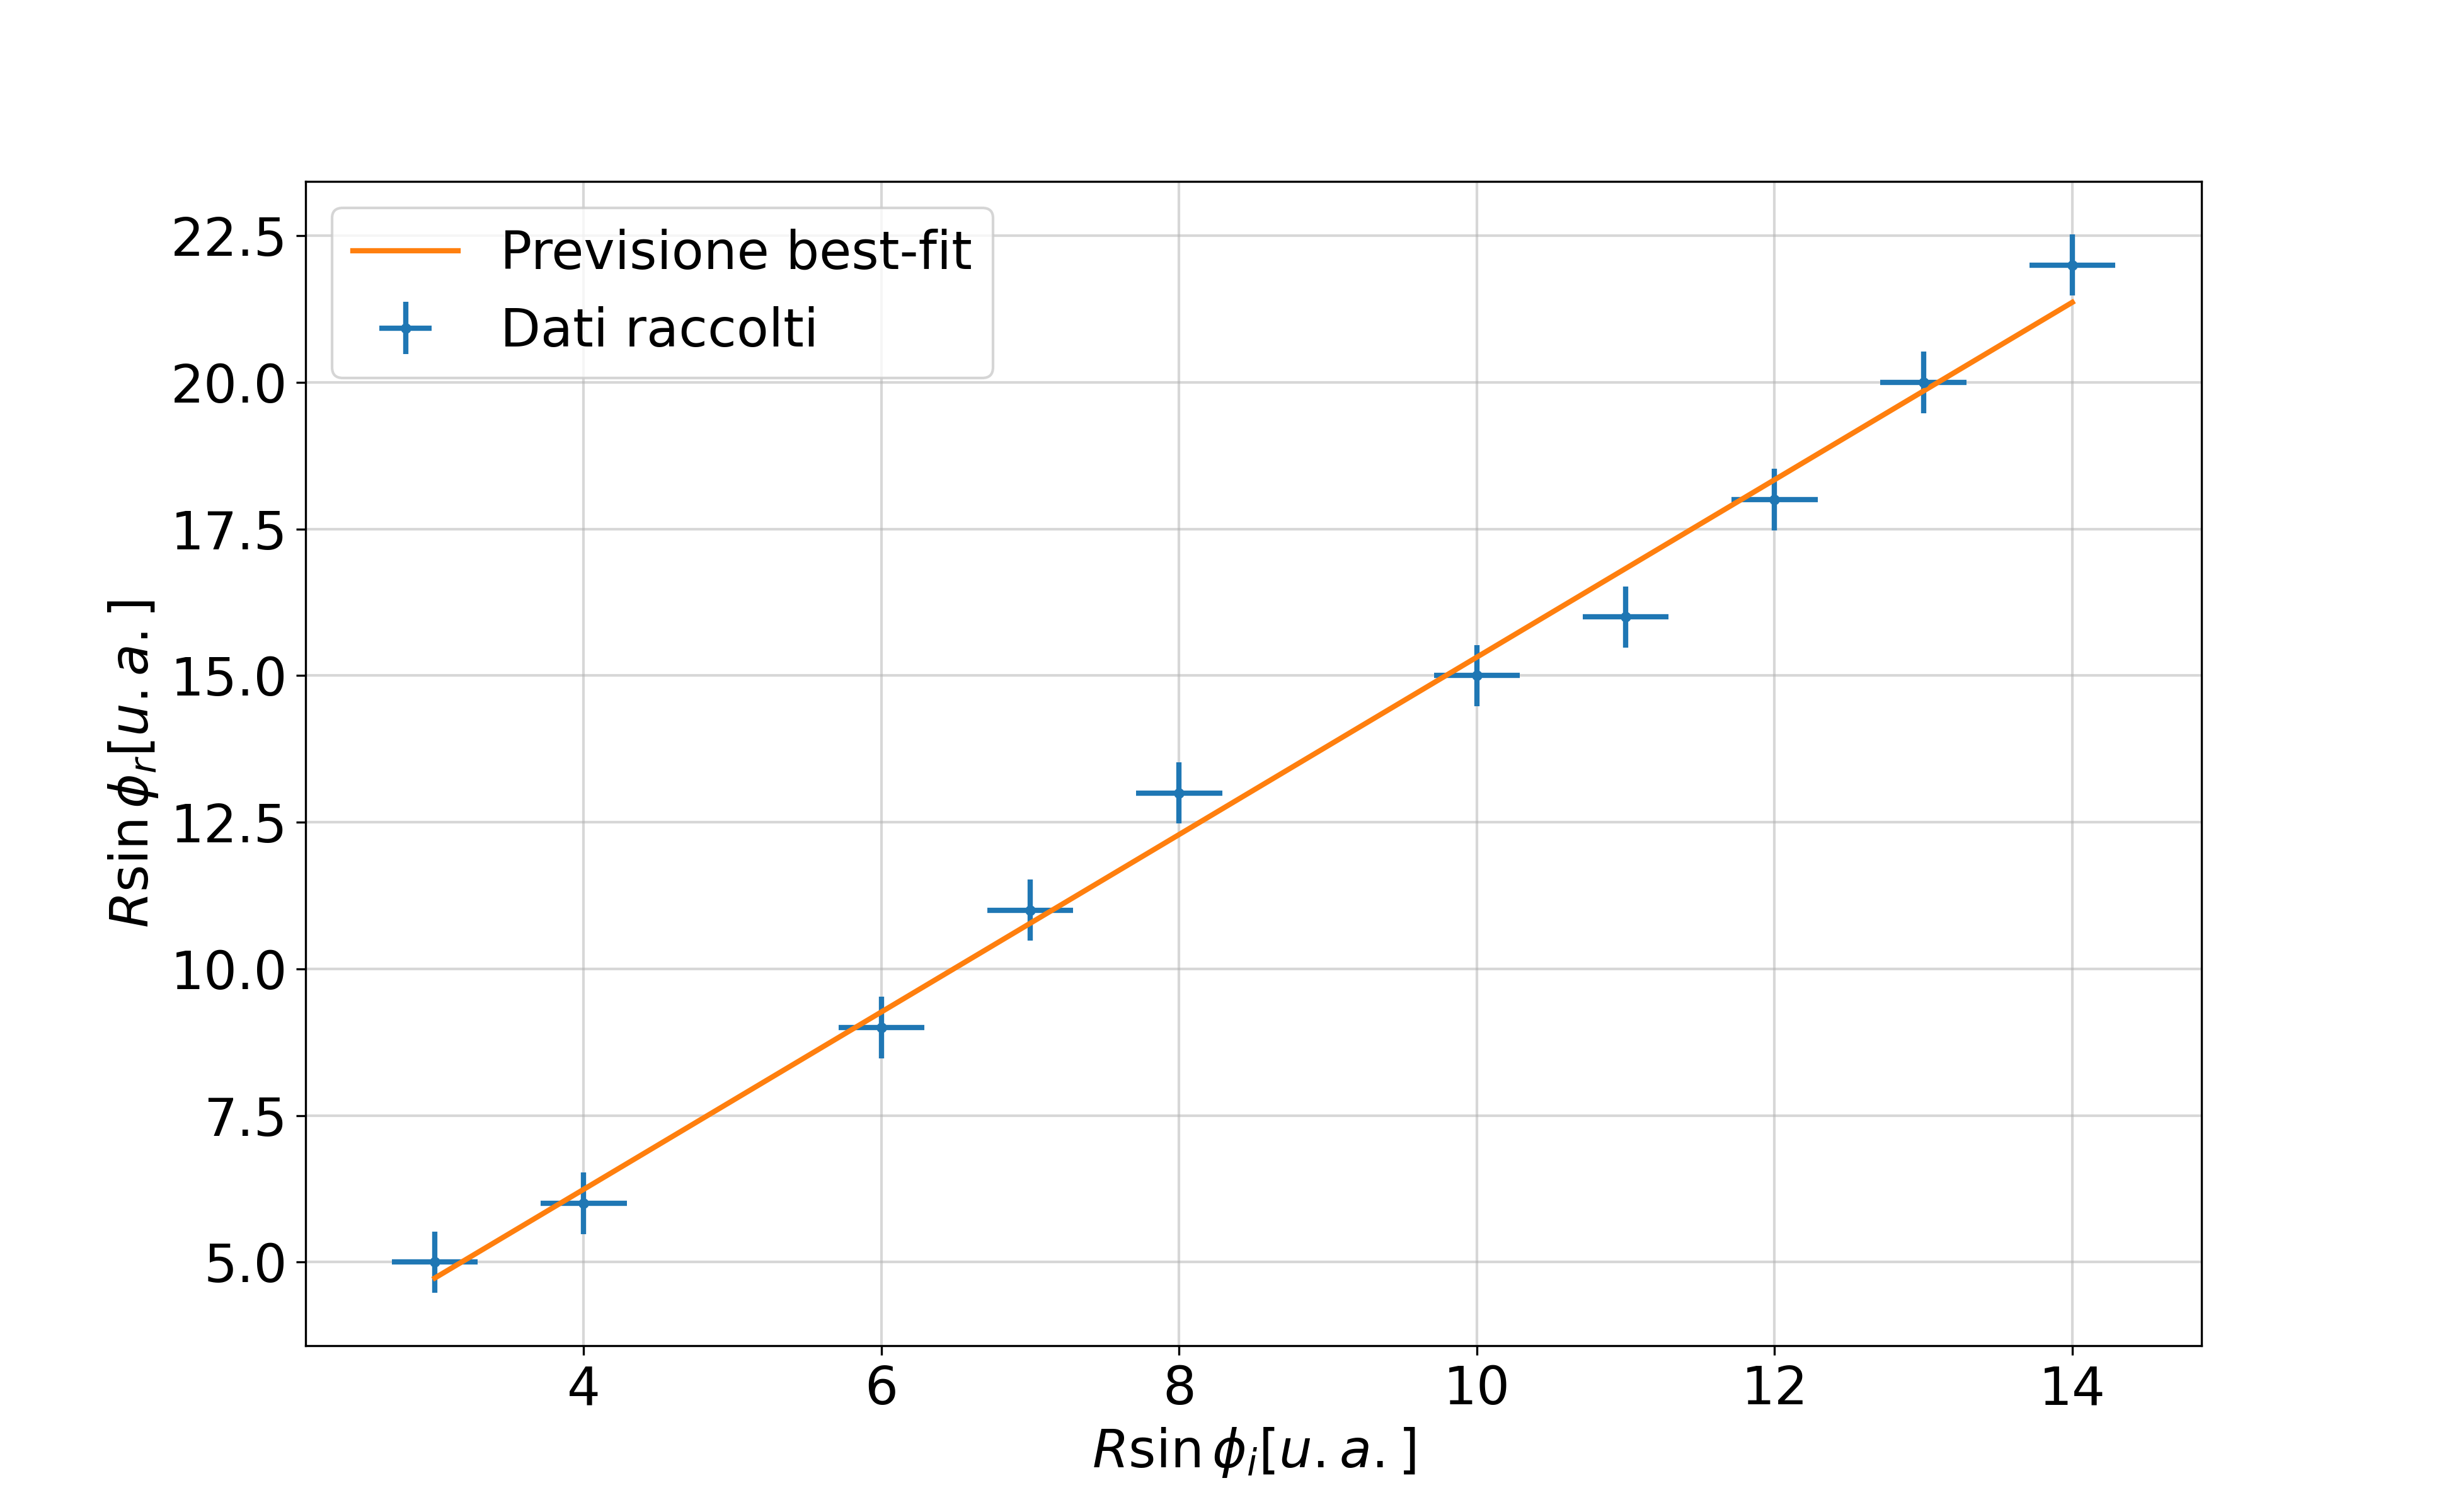
\includegraphics[width=\textwidth]{Dati_raccolti.png}
	\caption{Dati raccolti e grafico della legge(\ref{eq:lin}) con i parametri ottenuti dall'algoritmo di best-fit.}
	\label{fig:plex}
\end{figure}

\begin{figure}[H]
	\includegraphics[width=\textwidth]{Dati_raccolti_residui.png}
	\caption{Grafico dei residui della legge(\ref{eq:lin}).}
	\label{fig:plexres}
\end{figure}



\subsubsection{Valutazione del modello}

In accordo con la teoria l'intercetta è compatibile con 0.
Dal grafico dei residui non è evidente la presenza di errori sistematici.
Siccome $\chi^2= 7.6$, $p_{value}= 0.47$  e $Dof= 8$,  non vi è motivo rigettare il modello dell'equazione($\ref{eq::)}$).


\subsection{Misura della focale di una lente divergente}

Non essendo trascurabile l'errore sulla variabile indipendente sono stati usati gli errori efficaci.
E' stato fatto un algoritmo di best-fit con i minimi quadrati per la legge($\ref{eq::)}$).
Sono riportati in tabella($\ref{tab:len}$) i risultati dell'algoritmo di best-fit.
In figura($\ref{fig:len}$) sono riportati i dati raccolti e la previsione del modello teorico con i parametri ottenuti dall'algoritmo di best-fit.
In figura ($\ref{fig:lenres}$) è riportato il grafico dei residui.


\begin{table}[H]
		\centering
			\begin{tabular}{|cc|}
				\hline
				$c $[m$^{-1}$] & $ -2.9 \pm 0.3$\\
				$f$[m] & $0.32\pm 0.02$\\
				$m$ & $ 1.01 \pm 0.04$\\
				\hline
			\end{tabular}
		\caption{Valori ottenuti dall'algoritmo di best-fit per la legge (\ref{eq::)}).}
		\label{tab:len}	
\end{table}



\begin{figure}[H]
	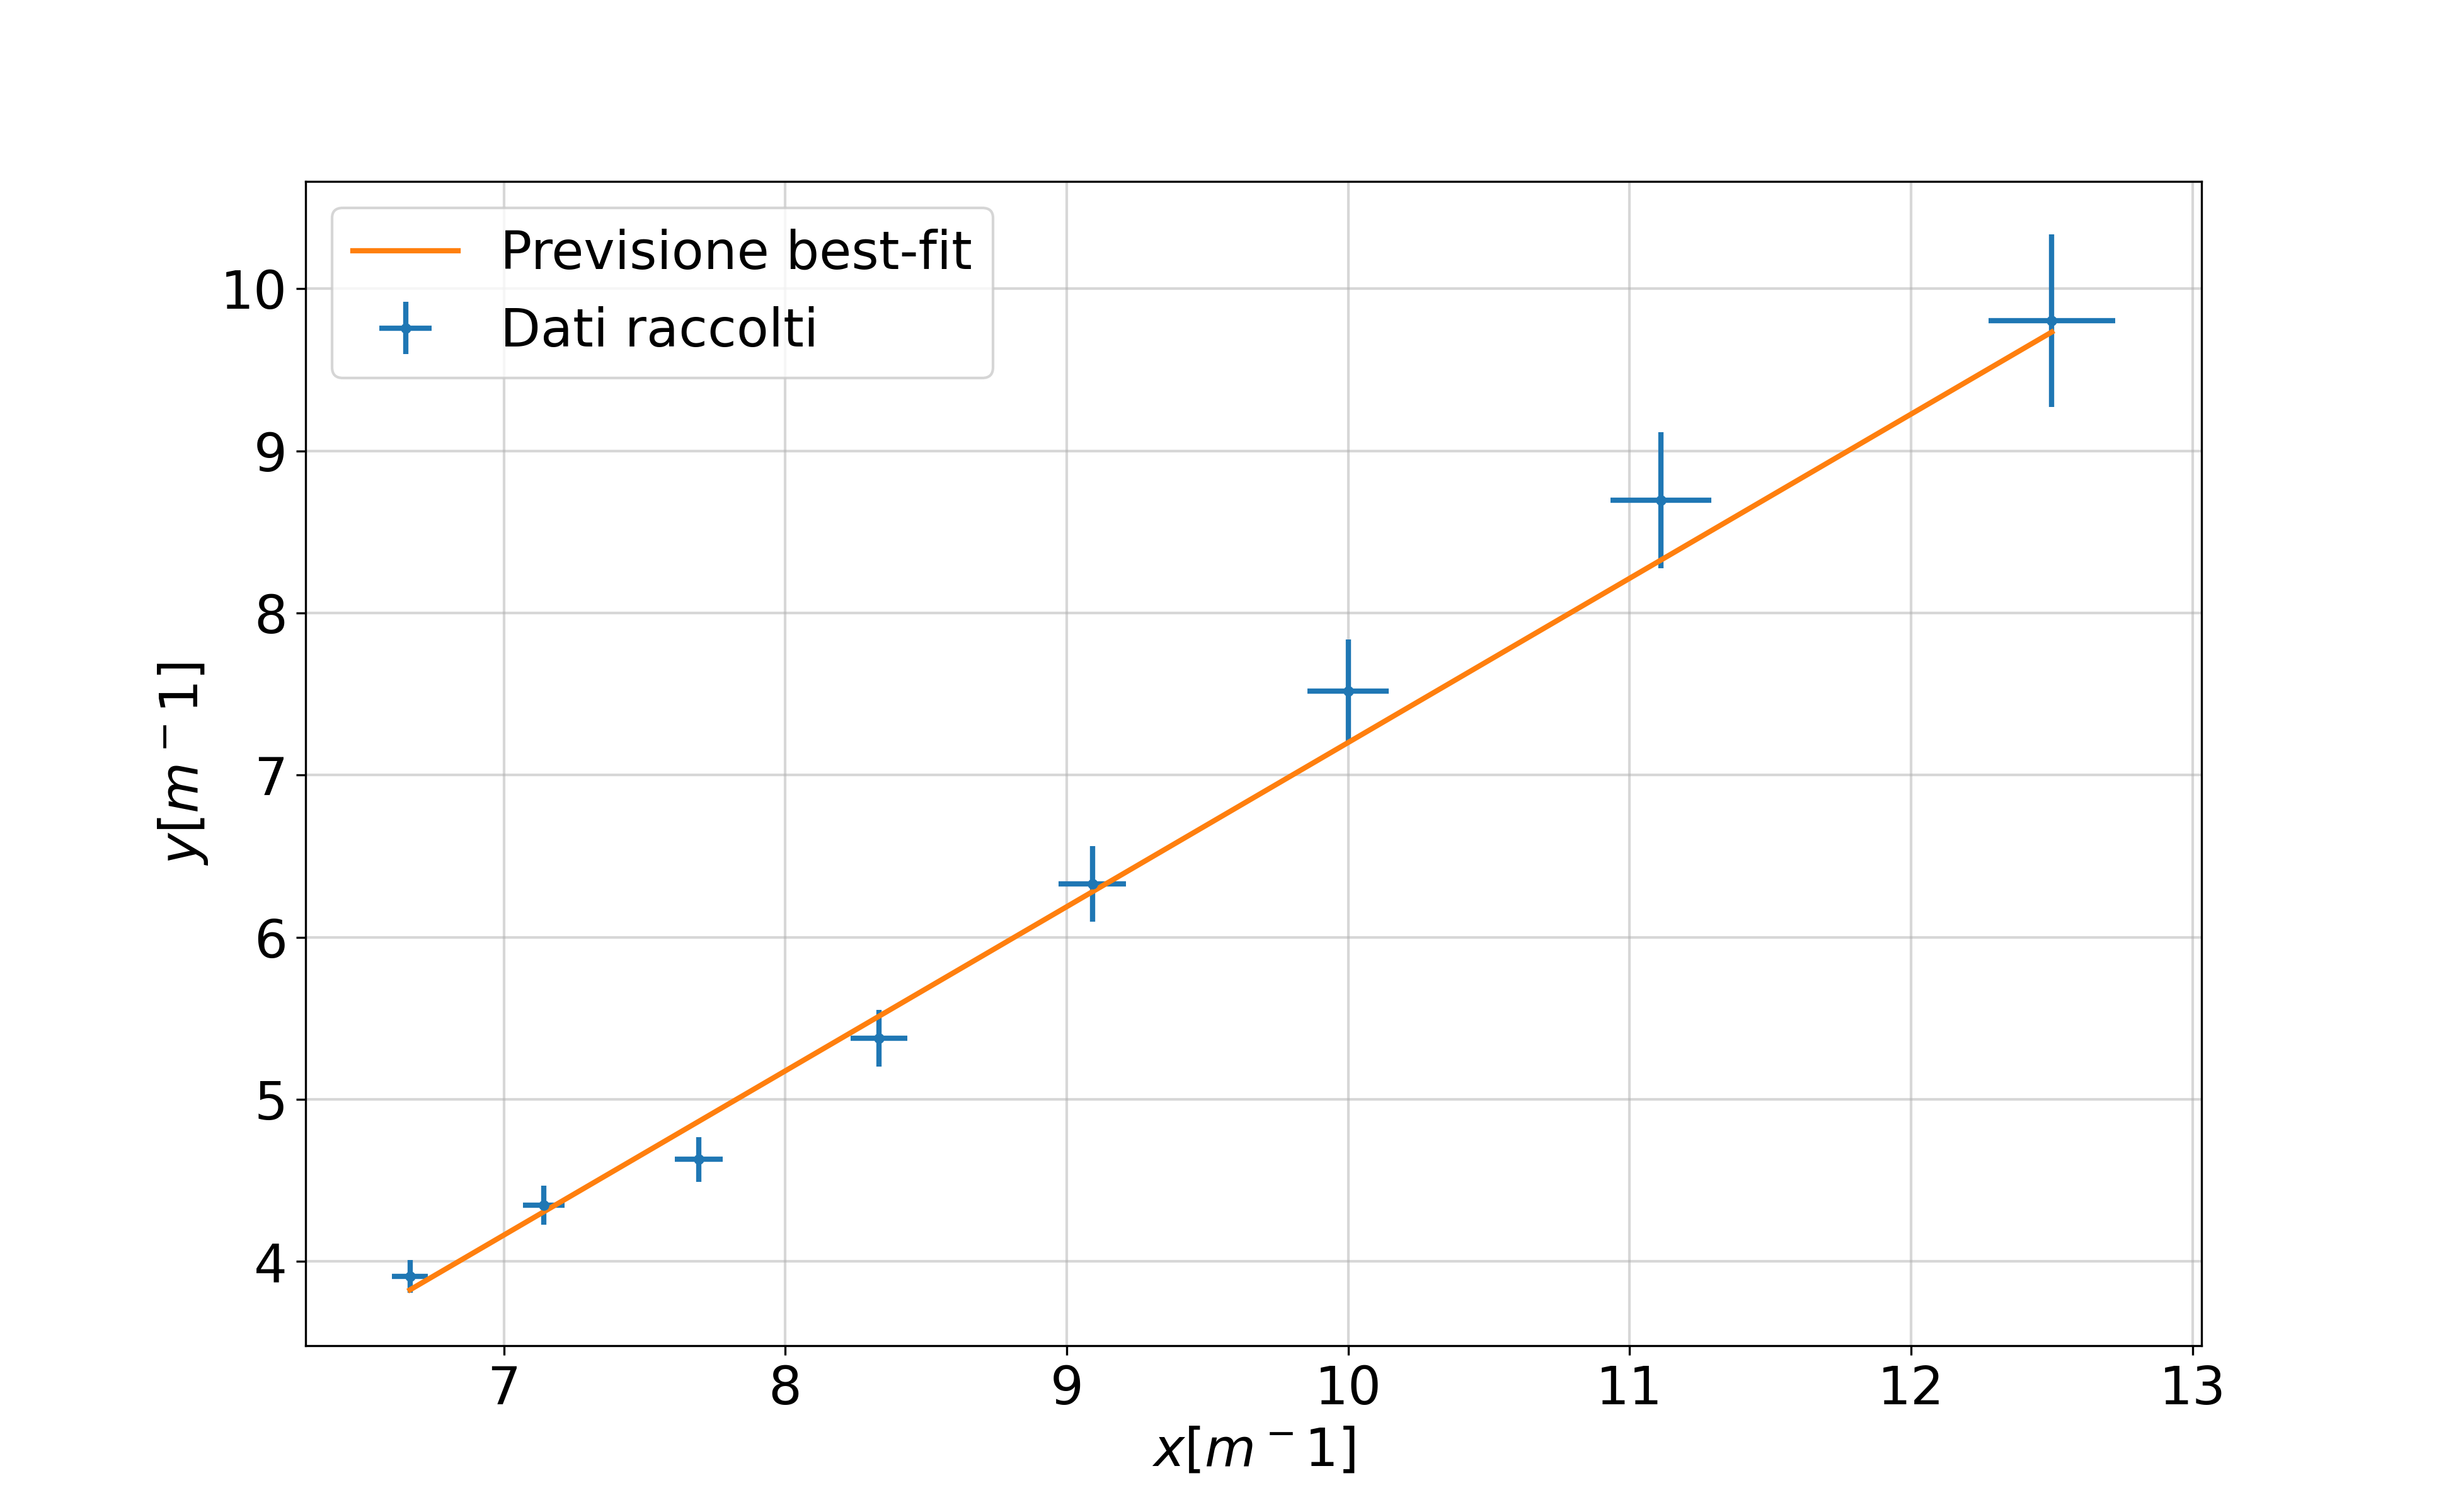
\includegraphics[width=\textwidth]{Dati_raccoltilen.png}
	\caption{Dati raccolti e grafico della legge(\ref{eq::)}) con i parametri ottenuti dall'algoritmo di best-fit.}
	\label{fig:len}
\end{figure}

\begin{figure}[H]
	\includegraphics[width=\textwidth]{Dati_raccolti_residuilen.png}
	\caption{Grafico dei residui della legge(\ref{eq::)}).}
	\label{fig:lenres}
\end{figure}

\subsubsection{Valutazione del modello}

In accordo con la teoria il coefficiente angolare $m$ è compatibile con 1.
Il grafico dei residui potrebbe suggerire un errore sistematico. La più plausibile causa è la messa a fuoco iniziale inesatta della lente convergente che si ripercuote su tutte le misure.
Siccome $\chi^2= 6.0$, $p_{value}= 0.4$  e $Dof= 6$,  non vi è motivo rigettare il modello dell'equazione($\ref{eq::)}$).


\section{Conclusioni}

E' stato misurato l'indice di rifrazione del plexiglas: $n_{plexiglass}= 1.51 \pm 0.03$ .
E' stato misurata la distanza focale della lente divergente: $f=0.32\pm0.02$ [m]

\end{document}